\documentclass[12pt]{article}
\usepackage{graphicx}
\usepackage{booktabs}
\usepackage{chngcntr}
\usepackage{pdfpages}

\usepackage{url}


\begin{document}

\pagenumbering{gobble}
\def\supervisorIname{Advisor I}
\def\supervisorIIname{Second Reviewer}

	\def\university{Universit\"{a}t des Saarlandes}
	\def\institute{Center for Bioinformatics}
	\def\chair{Chair for Clinical Bioinformatics}
	\def\projectname{MiRNA target analysis focussing on sequence alignment}
	\vspace{.2em}  
	\def\author{Louisa Schwed}
	\def\date{September 2016}

\begin{titlepage}

  \begin{minipage}{\textwidth}
    \begin{center}
    { \large Saarland University \\ Center for Bioinformatics \\ Chair for Clinical Bioinformatics \\}
	\vspace{0.5cm}
    
\includegraphics[width=4cm]{Logo-Universitaet_des_Saarlandes.pdf}\\
    \vspace{0.5cm}
    { \large Bachelor's Thesis\\}
    \vspace{0.5cm}
    {\huge\textbf{\projectname}}\\
    \vspace{0.5cm}
    { \large submitted by}\\
	\vspace{0.5cm}
    {\large\textbf{\author}}\\
    \vspace{0.5cm}
    {\large on September XX, 2016}\\
    \vspace{0.5cm}
    \end{center}
  \end{minipage}
  \newpage

    
    \begin{minipage}{\textwidth}
        \begin{center}
        \begin{minipage}{\textwidth}
        \begin{center}
		  \textbf{\emph{Supervisor}}\\
    		  \supervisorIname      \\
    		  \vspace{0.5cm}
		  \textbf{\emph{Advisors}}\\
    		 XXXX\\
    		  \vspace{0.5cm}
		  \textbf{\emph{Reviewers}}\\
		  \supervisorIIname \\
		  \vspace{0.5cm}
    		  Center for Bioinformatics\\
    		  
\includegraphics[scale=0.3]{cbi.jpg}	
              		          
    		  \end{center}
        \end{minipage}
		\hfill
     
        \end{center}
    \end{minipage}

\end{titlepage}


\newpage
\vfill
\pagestyle{empty}
\vspace{10cm}
\noindent {\bf Schwed, Louisa}\\
\emph{MiRNA target analysis focussing on sequence alignment}\\
Bachelor's Thesis in Bioinformatics\\
Saarland University
Saarbr\"ucken, Germany\\
September 2016
\newpage

\section*{Declaration}
\emph{I hereby confirm that this thesis is my own work and that I have documented all sources used.}

\vspace{1cm}

\noindent Saarbr\"ucken, September xx, 2016
\vspace{1.5cm}

\noindent Louisa Schwed
\newpage
\mbox{}



\tableofcontents

\newpage 
\pagestyle{plain}
\counterwithin{figure}{section}
\counterwithin{table}{section}

\bibliographystyle{apalike}
\pagenumbering{arabic}

\section*{Abstract}

blablabla
 
\section{Introduction}

miRNAs are small, non-coding RNAs that function in post-transcriptional regulation of gene expression, especially in terms of gene silencing. A miRNA consists of approximately 22 nucleotides which build a single strand RNA. The maturation of the miRNA is shown in figure~\ref{biogenesis}. After transcription the miRNA folds into a hairpin structure and builds the primary miRNA \cite{Macfarlane}. First, this pri-miRNA is processed by Drosha which results in a precursor miRNA (pre-miRNA). This precursor is about 60 to 70 nucleotides long and contains two single stranded miRNAs. After the export into the cytoplasm another processing step is executed with Dicer to gain the actual form of miRNA. But they are still double stranded and need to be unwinded to be mature miRNAs \cite{Macfarlane}. So after processing of the initial double stranded miRNA-duplex, the guide strand will be further used in association with other molecules \cite{Grunz}. In detail, the miRNA is mainly active in combination with a catalytic protein of the AGO protein family. With it, the miRNA builds an RNA-induced silencing complex \cite{Ha}. This complex targets a mRNA mainly at its 3' untranslated region (UTR) by complementary binding to the sequence. The miRNA functions in this case as a guide with their base pairing \cite{Macfarlane}. It can also bind at the 5' UTR or even in the coding region but these are the uncommon regions. Either way, this binding results in gene silencing either by repression of mRNA translation or degradation of the respective mRNA \cite{Enright}. Which of the two pathways is chosen depends on the degree of complementarity. As figure~\ref{biogenesis} illustrates, if the complementarity is nearly perfect then the target mRNA is degraded otherwise if the seed regions contains mismatches the translation is only repressed. Both ways have a huge impact on the expression and resulting genetic changes which can initiate cancer \cite{Macfarlane}.\\

\begin{figure}[h]
\centering
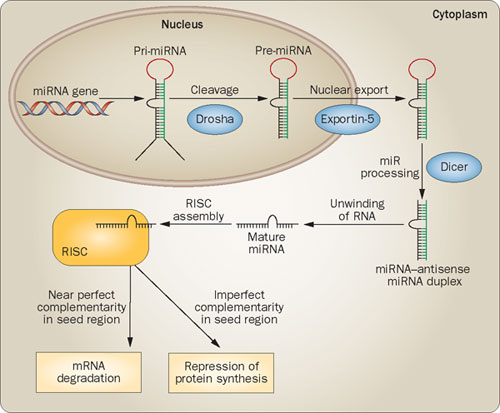
\includegraphics[scale=0.5]{results/biogenesis.png}
\caption{Biogenesis of miRNAs}
\label{biogenesis}
\end{figure}  

This gene regulation by miRNAs plays an important role for many major cell functions like growth, differentiation or metabolism and is currently examined by many investigators \cite{Ardekani}. The importance of miRNA and their regulation can also be observed by the fact that more than 60\% of all human genes have one conserved miRNA-binding site ore even more \cite{Ha}. Therefore disregulation, either up- or downregulation, may result in different human diseases, e.g. cancer or autoimmune diseases \cite{Ardekani}. Hence, this also leads to the assumption that miRNAs are a useful feature for the diagnosis and treatment of diseases. But they follow a very special and complicated targeting and this has to be elucidated. So the first step is to understand their function and regulation mechanism. With these information it can be possible to predict targets of miRNAs and then specifically effect these target interactions to diagnose or treat diseases. \\\\
But as already mentioned, especially this prediction of new targets of miRNAs is the main challenge in the whole field of miRNAs. There is still no perfect, reliable solution for it. There are a few tools that try to solve this problem. One of the first tools was miRanda. In their prediction algorithm they rely on three main features: sequence complementary, free energy and evolutionary conservation \cite{Enright}. Another tool is miRSVR that uses bit vectors and statistical learning approaches to predict targets. In this bit vector they store information like base complementarity, UTR length and distance, AU content and conservation \cite{Betel}. A third tool was developed called TargetScan. Their approach is based on seed matching and additional features like UTR positioning, AU content as well and base pairing of the 13nt to the 16nt miRNA nucleotide. They especially take the seed region into account by defining four different patterns of seed binding sites \cite{Lewis}.\\\\
The challenge of the prediction can be observed by considering the consensus of all predicted targets of the different tools.  Just a really small subset of all targets are predicted by all tools. If you then compare validated target interactions with the results of all tools about 16\% of all interactions are predicted by at least one tool. But there is no interaction that is predicted by all tools. That shows that there are big differences between the different tools partly because of the variable features they consider. (Quelle Keller Vorlesung 4) \\\\
Because the miRNA binds to the sequence of its target gene an obvious starting point can be the complementarity of the miRNA sequence to the gene sequence as almost each tool considers at first. The first thought could be that if the sequence complementarity is quite high this could be interpreted as a new target site. Considering the sequence alignment a high alignment score of miRNA and mRNA sequence can indicate a true target. Whether this is a reliable indication or not will be discussed below. For this assumption there already exist some problems beforehand. Because it is known that the main binding happens within the seed region, other regions are not necessarily complementary and this may lower the complementarity or alignment score. \\\\
Because of the early knowledge of base complementarity close to the 5'end of the miRNA, one of the first features that was used for the prediction, is the presence of the so called 'seed region' of the miRNA. This region consists of 7 or 8 nucleotides that are complementary to the respective nucleotides in the mRNA sequence. Another early characteristic is the bulge after the complementary region where the nucleotides do not fit together. After this part complementary bases towards the 3' end of the miRNA may occur again. Whether these rules apply and if they are present in validated data will be discussed later. \\\\
For these miRNA analyses three main databases are useful and necessary. A collection of experimental validated miRNA-target interactions(MTIs) is essential. The database miRTarBase provides a big dataset of validated MTIs \cite{Hsu}. To get information about every single miRNA for different organisms miRBase contains large datasets about the miRNAs. The most interesting information are sequences of the precursor and of all mature miRNAs \cite{mirbase}. For further analyses I will only consider miRNAs of \textit{Homo sapiens}. The last used database is the UCSC Genome Bioinformatics Site. In their table browser you can get data files about human gene sequences and untranslated regions and their respective sequences \cite{ucsc}.
  



\section{Methods and Data}


\subsection{Methodology}


only functional ones, not non and not weak
input data and runtime, csv etc.

The program for the analysis is implemented in Python. The data files are parsed and stored into dictionaries that allow fast searching. Then for every MTI in the miRTarBase file the respective miRNA sequence is searched in the miRBase file and combined with the gene sequence of the corresponding target in the UCSC file. The miRTarBase file contains data of Functional MTIs, weak Functional MTIs and Non-Functional MTIs. Here I only consider the strong validated data of the Functional MTIs because they deliver strong evidence for the interaction. 

Having theses two sequences, a local alignment is performed. An alignment is defined as the optimal positioning of the bases of one sequence, in this case the miRNA, to a region in the other sequence, the gene sequence. From the result functional or structural similarities can be obtained \cite{alignment}. In this case, the similarity can be interpreted as a binding site, because if we take the reverse complement of the miRNA sequence and align it to the mRNA sequence, this will simulate the binding. More precisely, if the alignment score is high, the sequences (mRNA and reverse complement of miRNA) are more similar, implying the actual miRNA could possibly bind at this alignment position. Because the miRNA can bind at any region in the gene, a local alignment is executed, not a global.\\\\

The Biopython library provides a module, pairwise2, for pairwise local alignments of two sequences. This tool is based on a dynamic programming algorithm. This function can be used either with default parameter or different scores and costs can be defined. The default parameters are as following: +1 for matching character, 0 for not matching ones and there are no gap penalties \cite{pairwise}. To get a more suitable alignment own parameters can be selected. Table~\ref{table:parameter} shows the different parameters that I used to generate the data. Set no. 8 is similar to the parameters they used for the tool miRanda \cite{Enright}. The other parameters are just logically selected to test which influence they have on the results. \\\\

To be able to analyse the data statistically a set of negative controls is required. To produce this data, 1000 miRNAs of the miRBase file were randomly assigned to a list of genes and then aligned in the same way as the sequences of the true target interactions. This randomly assigment can by chance contain true targets but generally the miRNAs are matched with genes that are no true targets. \\\\

For these datasets the average and standard deviation were computed as well. Then with case and control alignment scores a statistical two-tailed t-test for two samples with equal variances was performed with LibreOffice \cite{ttest}. This provides a p-value as a result. The lower this p-value is, the more significant the increase of the alignment score of the true targets is. If there is an increase in the score, this would be an indication that is we only calculate the alignment score for a new miRNA and any target sequence and observe a high one, the probability that this is a true target would be high. If this is a reliable feature for the prediction will be discussed in the following.

\begin{table}
\caption{Parameter sets}
\vspace{0.3cm}
\begin{tabular}{c|c|c|c|c}
Parameterset & match score & mismatch score & gap open & gap extend\\
\hline\hline 
1 & default: 1 & default: 0 & -4 & -4\\
2 &  default: 1 & default: 0 & -5 & -1 \\
3 &  1 & -2 & -2 & -1 \\
4 &  2 & -2 & -5 & -4 \\
5 &  3 & -2 & -4 & -4 \\
6 &  5 & -1 & -8 & -4 \\
7 &  5 & -2 & -8 & -3 \\
8 &  5 & -3 & -8 & -2 \\
9 &  5 & -4 & -6 & -4 \\
\hline
\end{tabular}
\label{table:parameter}
\end{table}

\subsection{Prediction features}
\subsubsection{Seed matching}
The main feature that is considered in this research is the sequence complementarity especially at a certain seed region. In contrast to miRNAs in plants which bind nearly perfectly complementary to their targets, miRNAs in animals bind less tightly and are not perfectly complementary. There can be regions were the nucleotides are unbound which results in complex secondary structures that are hard to predict \cite{Rehmsmeier}. The main complementary region or seed region includes nucleotides from position two to eight starting from the 5' end. Figure~\ref{seed} shows the scheme of the seed region \cite{Peterson}. This irregularity of the presence of non-complementarity regions makes the reliable prediction more difficult for animals than for plants. Because concentration on the seed region for a prediction will lead to many false positives. This small region of seven or eight nucleotides would be too unspecific because they can be present in the mRNA although there is no binding site at this position. It would be recommended to take more than the seed region into account to increase the complexity and specificity of the prediction. How significant the consideration of the sequence complementarity of miRNA and mRNA sequence is, will be further analysed with validated data in this research.\\\\
In the mentioned seed region there can be different types of matching patterns: perfect matching between six nucleotides, seven nucleotides including the 8th position, seven nucleotides and an Adenine at position one or eight matching nucleotides from position one to eight and also an Adenine at position one  \cite{Lewis} \cite{Brennecke} \cite{Krek}. Figure~\ref{Fig:canonical} illustrates the different types of sites. Grimson et al. \cite{Grimson} investigated the different types of sites referring to the effectiveness of the gene repression. As shown in figure~\ref{types}, they found that the repression is the highest when an 8mer site is present and the lowest when only six nucleotides are perfectly matching.


\begin{figure}[h]
\centering
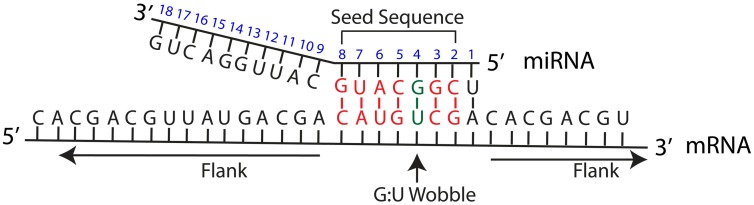
\includegraphics[scale=2.8]{results/seedmatching.png} 
\caption{Scheme of seed matching}
\label{seed}
\end{figure}


\begin{figure}
\centering
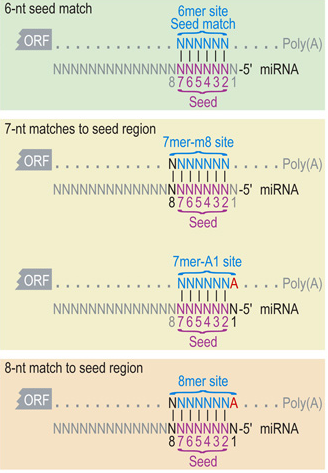
\includegraphics[scale=0.6]{results/canonical_sites.png}
\caption{Canonical sites of seed region}
\label{Fig:canonical}
\end{figure}


\begin{figure}
\centering
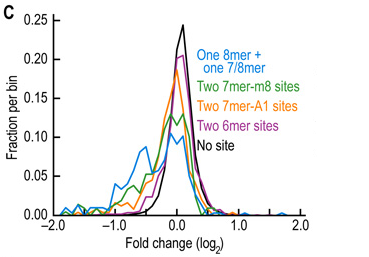
\includegraphics[scale=0.6]{results/site_3addi.png}
\caption{Effectiveness of different types of sites}
\label{types}
\end{figure}

\subsubsection{Free energy}
The free energy of a system determines its stability and tightness of binding. If the free energy is lower than the binding between the miRNA and the mRNA sequence is tighter resulting in more evidence that this miRNA targets this mRNA. If the energy is high then the binding is not very favourable meaning the miRNA not favours to target this mRNA at this position. Some tools like RNAhybrid \cite{Rehmsmeier} rely mainly on this feature. (thermodynamics von miranda)
 
\subsubsection{Conservation}
Another feature to take into account is the evolutionary conservation. If a sequence occurs across species it is defined as conserved. This implicates that this part has been maintained by evolution because of a selected function \cite{Peterson}. Conservation near the miRNA binding site can indicate that this part of the sequence is necessary for some mechanisms. This includes conservation of the miRNA itself as well as the conservation of the respective site of the mRNA. These conservations can be analysed with phylogenetic methods. In terms of conservation, figure~\ref{conserved} shows how conserved the different nucleotides of a miRNA are implicating regions like the seed region and additional 3' pairing. 


\subsubsection{Site accessibility}
Kertesz et al. \cite{Kertesz} investigated the importance of site accessibility for the target prediction. The mRNA generally folds into a secondary structure. Therefore the miRNA can not easily bind to its target because at first, interactions within the mRNA have to be broken to make the target accessible. As a result miRNA will favourably bind to regions where the mRNA is more accessible. Kertesz et al. \cite{Kertesz} found that if the targets form highly stem structures the repression is reduced. If sites occur in open loop structures the repression is much higher. Summing up they found that site accessibility is not less important than seed matching. \\


\subsubsection{Addtional Watson-Crick pairing}
In addition to the seed matching towards the 5' end, another complementary site towards the 3' end in the miRNA is present (Figure~\ref{addipairing}). Grimson et al. \cite{Grimson} investigated that the highest down regulation was found when the site started at position 13 and had four or five contiguous base pairings (Figure~\ref{siteregulation}). Considering again the conservation of the nucleotides they found that outside the seed region the contiguous nucleotides starting from nucleotide 12, 13 or 14 were the most conserved ones indicating / demonstrating their functional importance (Figure~\ref{conserved}). Putting the information of seed region and additional base pairing together, it can be observed that if one 7mer-m8 site is present as well as a good 3' pairing that the efficacy is the highest. Even though the difference between the efficacy of the presence of one 8mer site and the one mentioned before is not very big. But the improvement of the presence of a good 3' pairing instead of a poor one is more significant (Figure ~\ref{efficacy}).  \\\\
Between the two complementary areas there is usually a part of non pairing nucleotides where bulges and mismatches are found. These are important for the prevention of the AGO cleavage function \cite{Filipowicz}.

\begin{figure}
\centering
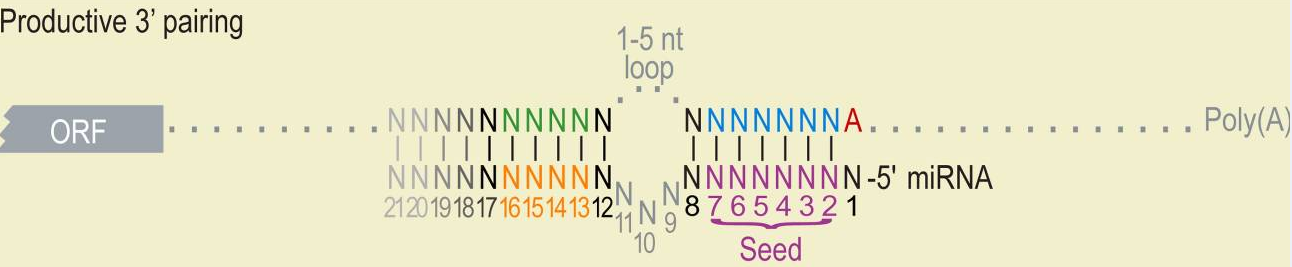
\includegraphics[scale=0.3]{results/additional_pairing.PNG}
\caption{Additional 3' pairing}
\label{addipairing}
\end{figure}

\begin{figure}
\centering
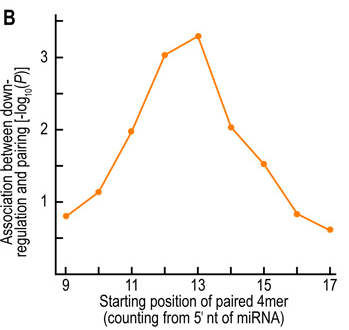
\includegraphics[scale=0.4]{results/sites_regulation.PNG} 
\caption{Relation between regulation and starting position of additional pairing}
\label{siteregulation}
\end{figure}

\begin{figure}
\centering
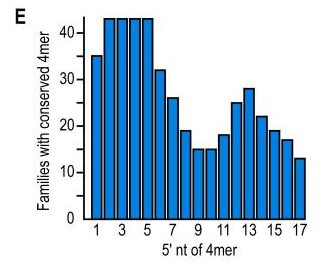
\includegraphics[scale=0.5]{results/sites_conserved.PNG} 
\caption{Conservation of nucleotide positions of miRNA}
\label{conserved}
\end{figure}

\begin{figure}
\centering
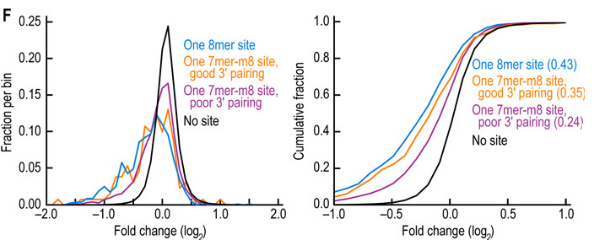
\includegraphics[scale=0.5]{results/site_efficacy.PNG} 
\caption{Efficacy of different combinations of seed region and additional 3' pairing}
\label{efficacy}
\end{figure}



\subsubsection{Other features}
To get an even more reliable and precise prediction additional features can be considered. The presence of GU-wobbles is common in targeting. In this wobble positions Guanine(G) binds to Uracil(U) even though the pairing with Cytosine would be prevalent. This special pairing is thermodynamically favourable and occurs therefore in many target interactions but results in lower repression of the translation \cite{Doench}. As mentioned before miRanda uses different scores for matches in their alignment step. They score the usual base pairing A-U and G-C with +5 and they penalize the other mismatches with a score of -3, excluding the pairing of G and U. This pairing is rewarded with at least +2 and therefore the GU wobbles are not penalized as much as other mismatches because they are very common \cite{Enright}.\\\\
 
https://elifesciences.org/content/4/e05005

Enright et al. \cite{Enright} and Doench et al. \cite{Doench} also found that the presence of multiple miRNA target sites results in a higher repression and destabilization of the mRNA. Grimson et al. \cite{Grimson} further investigated that the distance between two sites is also an important criterion. Generally the repression of two present site is the multiplication of the two single once because they act independently. The interesting thing now is that if the two sites are adjacent the repression is increased and not equal to the multiplication of the single ones. The increase in repression is however not very high (Figure~\ref{sitedistance}). To investigate the effect of cooperative miRNAs they analysed a mixture of miR-1 and miR-133 and simulated three different spacings. The results show that a spacing of four nucleotides did not show a cooperative repression but six or eight nucleotide spacing showed an increase in repression (Figure~\ref{sitespacing}).\\\\

\begin{figure}
\centering
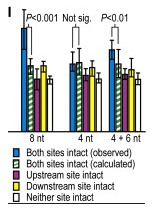
\includegraphics[scale=1.2]{results/sites_8nt.PNG}  
\caption{Cooperative repression with different site spacings}
\label{sitespacing}
\end{figure}

\begin{figure}
\centering
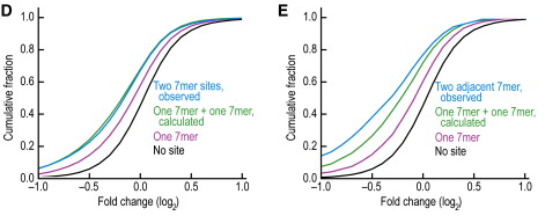
\includegraphics[scale=0.7]{results/sites_distance.PNG}
\caption{Effect of multiple sites}
\label{sitedistance}
\end{figure}

Another indicator is the position of the binding site relatively to the stop codon and the center of the UTR. Generally sites in the 3'UTR are investigated but Grimson et al. detected that sites in the Open reading frame (ORF) are slightly effective, sites in the 5'UTR not at all \cite{Grimson}. \\\\

\begin{figure}
\centering
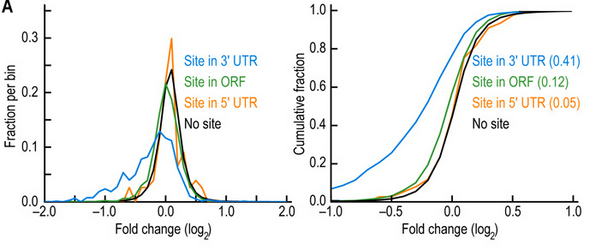
\includegraphics[scale=0.7]{results/sites_orf.PNG}
\caption{Efficacy of different site locations}
\label{siteorf}
\end{figure}

Figure~\ref{siteorf} shows the different efficacies. Another characteristic concerning the site locations is the distance from the stop codon. Figure~\ref{sitestop} illustrates that approximately in the first 15 nucleotides the efficacy is still very low like in the ORF but afterwards it increases much. 
The sites were present at least 15 nucleotides from the stop codon and not present in the center of long UTRs but away from it. \\\\

Grimson et al. also found that the AU nucleotide content is increased in the region of conserved sites \cite{Grimson}.

\begin{figure}
\centering
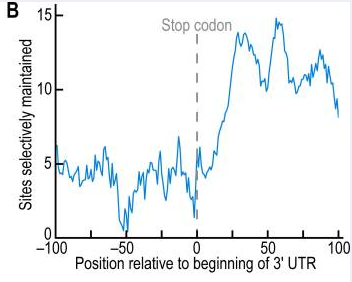
\includegraphics[scale=0.6]{results/site_stop.PNG} 
\caption{Efficacy of sites located relative to the stop codon}
\label{sitestop}
\end{figure}

   
Considering all these different common and less common features, new targets for miRNAs can be roughly reliably predicted. Figure~\ref{fig:tools} shows known prediction tools and the features they consider. As mentioned above the most common feature that nearly all of them consider are seed matching, conservation and free energy. 


\begin{figure}
\centering
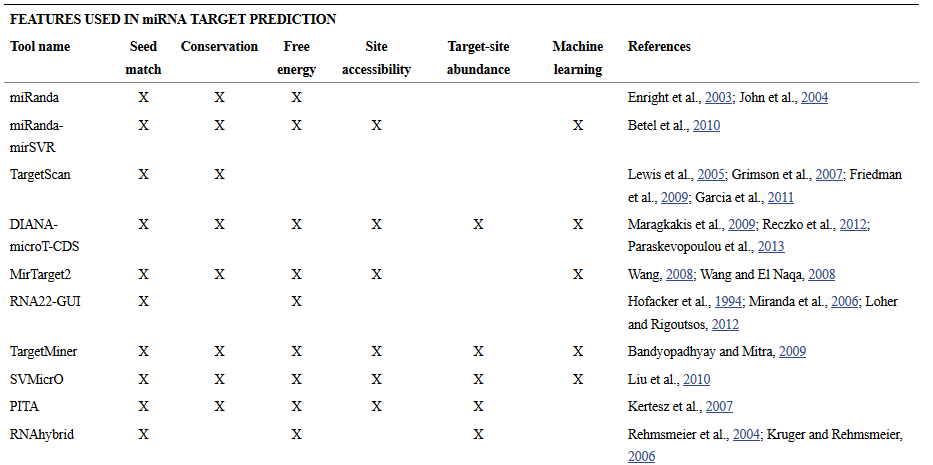
\includegraphics[scale=0.5]{results/tools.PNG}
\caption{Prediction tools and their features}
\label{fig:tools}
\end{figure}

 
\subsection{Data} 
\subsubsection{miRTarBase}
The database mirTarBase which was released in 2010 provides by now about 7500 strong validated MTIs and 348000 weak ones from different species \cite{Chou}. In this research I concentrate on humans. Different experiment types were used to validate the data, including Reporter assay, Western plot, qPCR, Microarray, NGS, pSILAC and other methods where the first three are the ones that deliver strong evidences \cite{Hsu}. Again in here, I only concentrate on the strong evidence targets. In detail, the data collection provides many information about the interaction between one miRNA and its target. Interesting details are the predicted alignments of miRNA and target 3' UTR sequence by either the author of the MTI or other prediction tools like miRanda. These alignments will also play an important role in the following analyses. From the database catalogue you can directly download the respective MTI data tables of the favoured species, in this case \textit{Homo sapiens}. The table then contains the following information: miRTarBase ID, miRNA name, species of the miRNA, target gene symbol, target gene Entrez ID, species of the target gene, experiment type, support type, references. The interesting fields for the research are name of the miRNA, the target gene ID and the experiment type because I only concentrate on the Functional MTIs that are not weak. In fact, every single strong validated interaction was analysed.\\\\

As mentioned above, the miRTarBase provides also binding sites as alignment positions predicted by different tools. To decide whether my own found alignments are compatible with the provided ones, the miRTarBase html page was parsed to get the start positions of each provided alignment. These positions exist not for every miRNA but for about 3700 of the interactions. The parsed positions can then be compared to the resulting positions by the pairwise2 module. 

\subsubsection{miRBase}
To get the corresponding sequence of the miRNA name, miRBase, which was already published in 2005, provides a complete dataset of all known miRNAs \cite{Griffiths-Jones}. By now it contains about 35000 mature forms and 2500 of it are found in \textit{Homo sapiens}. The table with all miRNAs includes the accession number, miRNA ID, status, sequence, accession number of first mature form, its ID, its sequence, accession number of the second mature form, its ID and its sequence. I only use the of the IDs and the sequences to align those to the gene sequence \cite{mirbase}.

 
\subsubsection{UCSC Genome Bioinformatics Site}
The last required dataset is the collection of target gene sequences and their respective untranslated regions (UTRs). On the UCSC Genome Bioinformatics Site you can generate a list of all genes and their UTRs of the human genome using the Table Browser \cite{ucsc}. The list consists of a description of the gene with the transcript accession number (NM-number) and the concatenated sequences of 5'-UTR, gene and 3'-UTR.\\\\

For the alignment of miRNA to the corresponding gene the respective miRNA sequence and gene sequence are required. The interaction data from miRTarBase only provides the correlation between miRNA name and target gene ID. But the dataset from UCSC only delivers the NM number for the gene sequence. Therefore a conversion from gene Entrez ID to Refseq mRNA accession number is required. Biodbnet provides a conversion tool for different IDs, names and numbers \cite{biodb}. I entered all existing target Entrez IDs of the miRTarBase file and obtained a list of IDs and their corresponding Refseq accession numbers. In my program I used this list by storing every entry in a dictionary and simply looked the particular ID up for every MTI. 
 


\section{Results}
For each parameter set the alignment score for every MTI is stored in a table. Additionally the average alignment score, the standard deviation and the p-values are listed underneath. Table~\ref{table:results} shows only a summary of the table, excluding the single alignment scores. (whole table somewhere else) To draw a better comparison, the scores of the non targets are listed right under the scores of the true targets. The averages of both alignment score sets show that the scores of the true targets are in general only slightly higher than the ones of the non targets. For the lower alignment scores of e.g. set 1 -2 -2 -1, resulting from really low match scores, the difference is only 0.3, so not very significant. For the higher scores, the difference amounts to 2. The standard deviation of the non targets is slightly higher than for the true targets but also not very significant. The p-value sheds light on whether the increase in the alignment score is significant when considering the whole set of scores. According to the listed values of the t-test this is a significant increase in the score because they are all really low. The parameters 5 -1 -8 -4 show the most significant difference with a p-value of 2.529E-61 whereas 2 -2 -5 -4 shows the least significant increase but also here the p-value is really low with 3.279E-36. So even though the average scores are not significantly different, the scores of the true targets seem to be distributed in the higher scores and the ones of the non targets in the lower scores.

\begin{table}
\footnotesize
\caption{Table of alignment results}
\vspace{0.3cm}
\begin{tabular}{c|c|c|c|c|c}
& 3 -2 -4 -4 & 5 -1 -8 -4 & 5 -2 -8 -3 & 5 -3 -8 -2 & 5 -4 -6 -4 \\
\hline\hline
Average true targets & 33.096 & 64.247 & 59.495	& 56.391 & 55.510\\
Average	non targets & 31.831 & 62.199 & 57.464 & 54.269 & 53.294 \\
\hline
Standard deviation true targets & 4.058	& 5.758 & 6.304	& 6.633 & 6.806\\
Standard deviation non targets & 4.233 & 6.510 & 6.753 & 6.876 & 7.01\\
\hline
t-test p-value & 5.934E-49 & 2.529E-61 & 1.040E-51 & 1.394E-51 & 1.744E-53 \\\hline
\end{tabular}\vspace{0.5cm}


\begin{tabular}{c|c|c|c|c}
& -4 -4 & -5 -1 & 1 -2 -2 -1 & 2 -2 -5 -4  \\
\hline\hline
Average true targets & 13.712 & 13.710 & 8.593 & 18.351\\
Average	non targets & 13.362 & 13.361 &	8.208 &	17.619 \\
\hline
Standard deviation true targets & 1.078	& 1.078	& 1.347	& 2.751\\
Standard deviation non targets & 1.311 & 1.309 & 1.385 & 2.868\\
\hline
t-test p-value & 8.824E-50 & 1.131E-49 & 8.157E-42 & 3.279E-36 \\
\hline
\end{tabular}
\label{table:results}
\end{table}

This increase in the alignment score can be also be observed when considering the distribution of the scores within the two groups of case and control. For two parameter sets (No. 1 and no. 8) such a distribution was plotted which is shown in figure~\ref{fig:distribution}. 

\begin{figure}
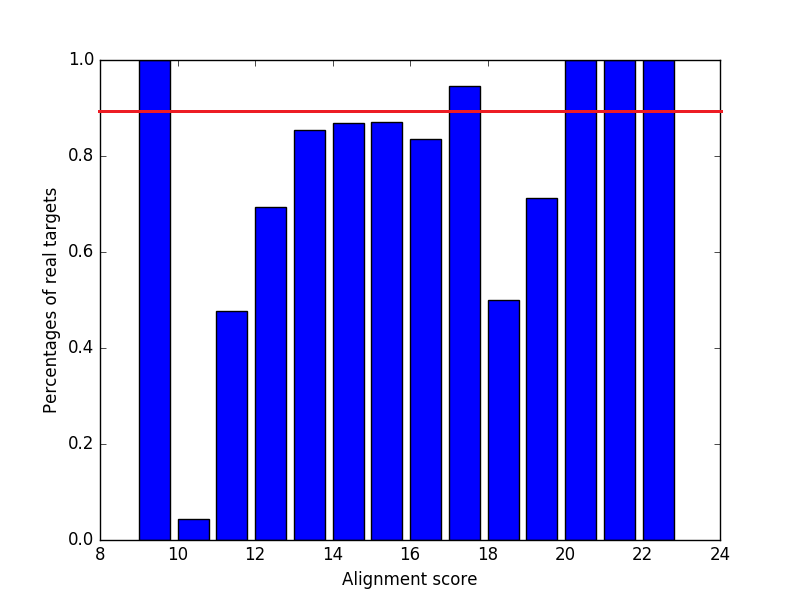
\includegraphics[scale=0.35]{results/plot_scores-4-4_thresh.png}
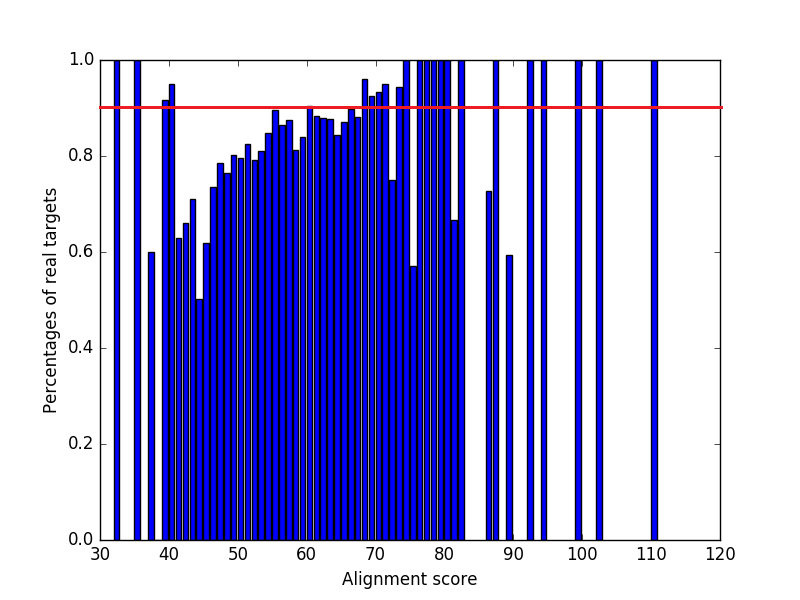
\includegraphics[scale=0.35]{results/plot_scores5-3-8-2_thresh.png}
\caption{Distribution of alignment scores, parameters -4 -4 and 5 -3 -8- 2}
\label{fig:distribution}
\end{figure}

On the x-axis the different existing scores of the respective data set are shown and on the y-axis the percentage of how many of the true targets had these scores. It can be observed that towards the higher alignment scores the percentage of true targets with this score increases. But also, there are some scores that are exceptions because more non targets produced this scores than true targets shown by lower y-values. Using this score as a prediction feature, a certain threshold needs to be determined to identify a true target. In figure~\ref{fig:distribution} a threshold of 90\% is delineated meaning at least 90\% true targets produced a certain alignment but still 10\% of random non targets had this score as well. Assuming this threshold and using the alignment scores for a prediction, for the first parameter set if we have scores of nine, 17, 20, 21, 22 or 23, a mRNA would be classified as a true target. Obviously the score nine would not fit in the pattern because it is a really low alignment score and the binding site would not be very suitable. On the other hand, alignments of miRNA and mRNA with a resulting score or 19 which belongs to the higher scores for this set, would not be classified as a true target even though the binding might be good. How this classification will look like depends strongly on this threshold. A lower threshold will result in a higher lower specificity and higher sensitivity, a higher one vice versa, so the two measurements of the performance need to be balanced.

For the second plot the same can be observed: some lower alignment score are above the threshold although they are not suitable and for some higher ones the probability to be a true target would be low.

Summing up, assuming the score as the only prediction feature and given a certain threshold, some mRNAs are predicted right to be true targets but there are also false positives. Given high alignment scores, a true target is not necessarily present. This uncertainty can be compensated by considering many more features to combine them and get a more reliable prediction.\\ 


For each parameter set the complementarity of single nucleotides of the alignments of miRNA and target gene sequence were also plotted. These plots are shown in figure~\ref{ratios}.

\begin{figure}
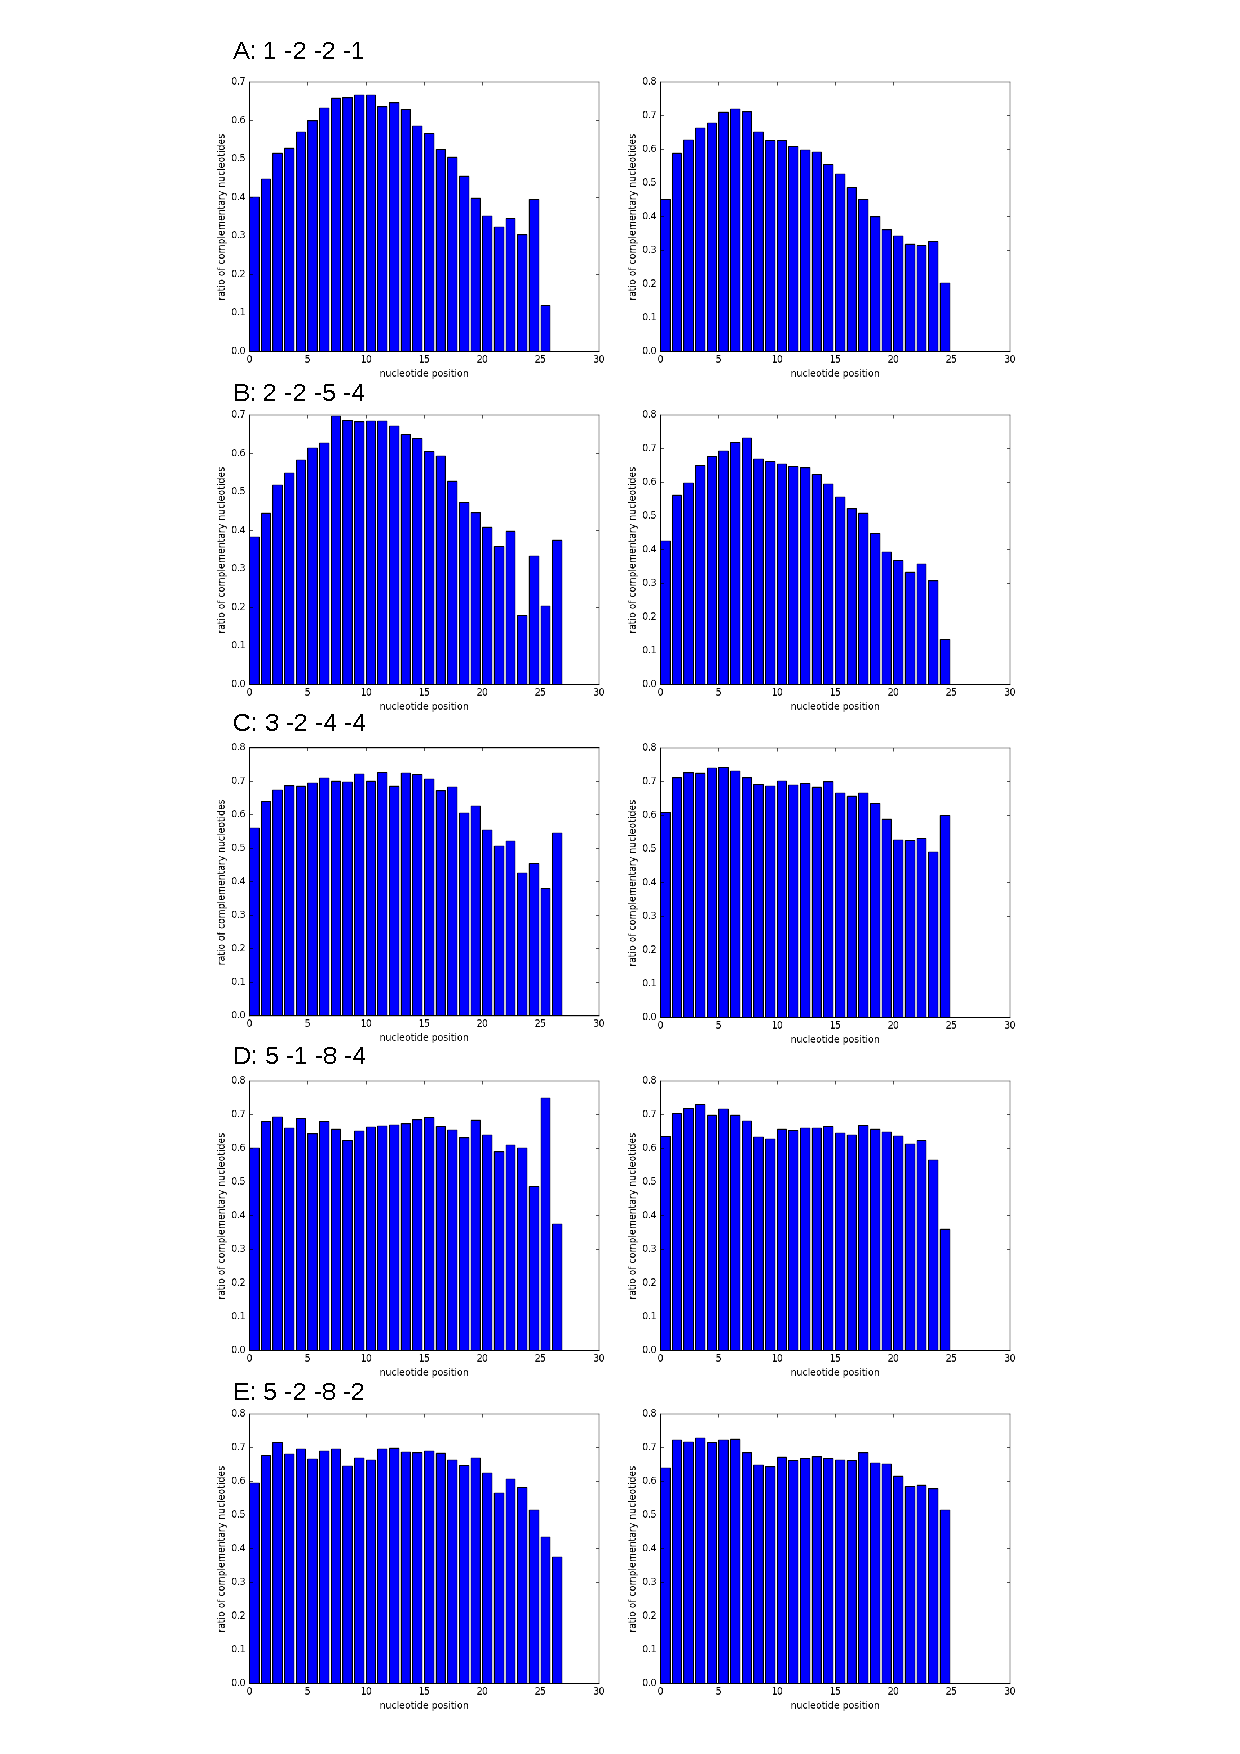
\includegraphics[scale=0.65]{results/combined_results.pdf}

\end{figure}

\begin{figure}
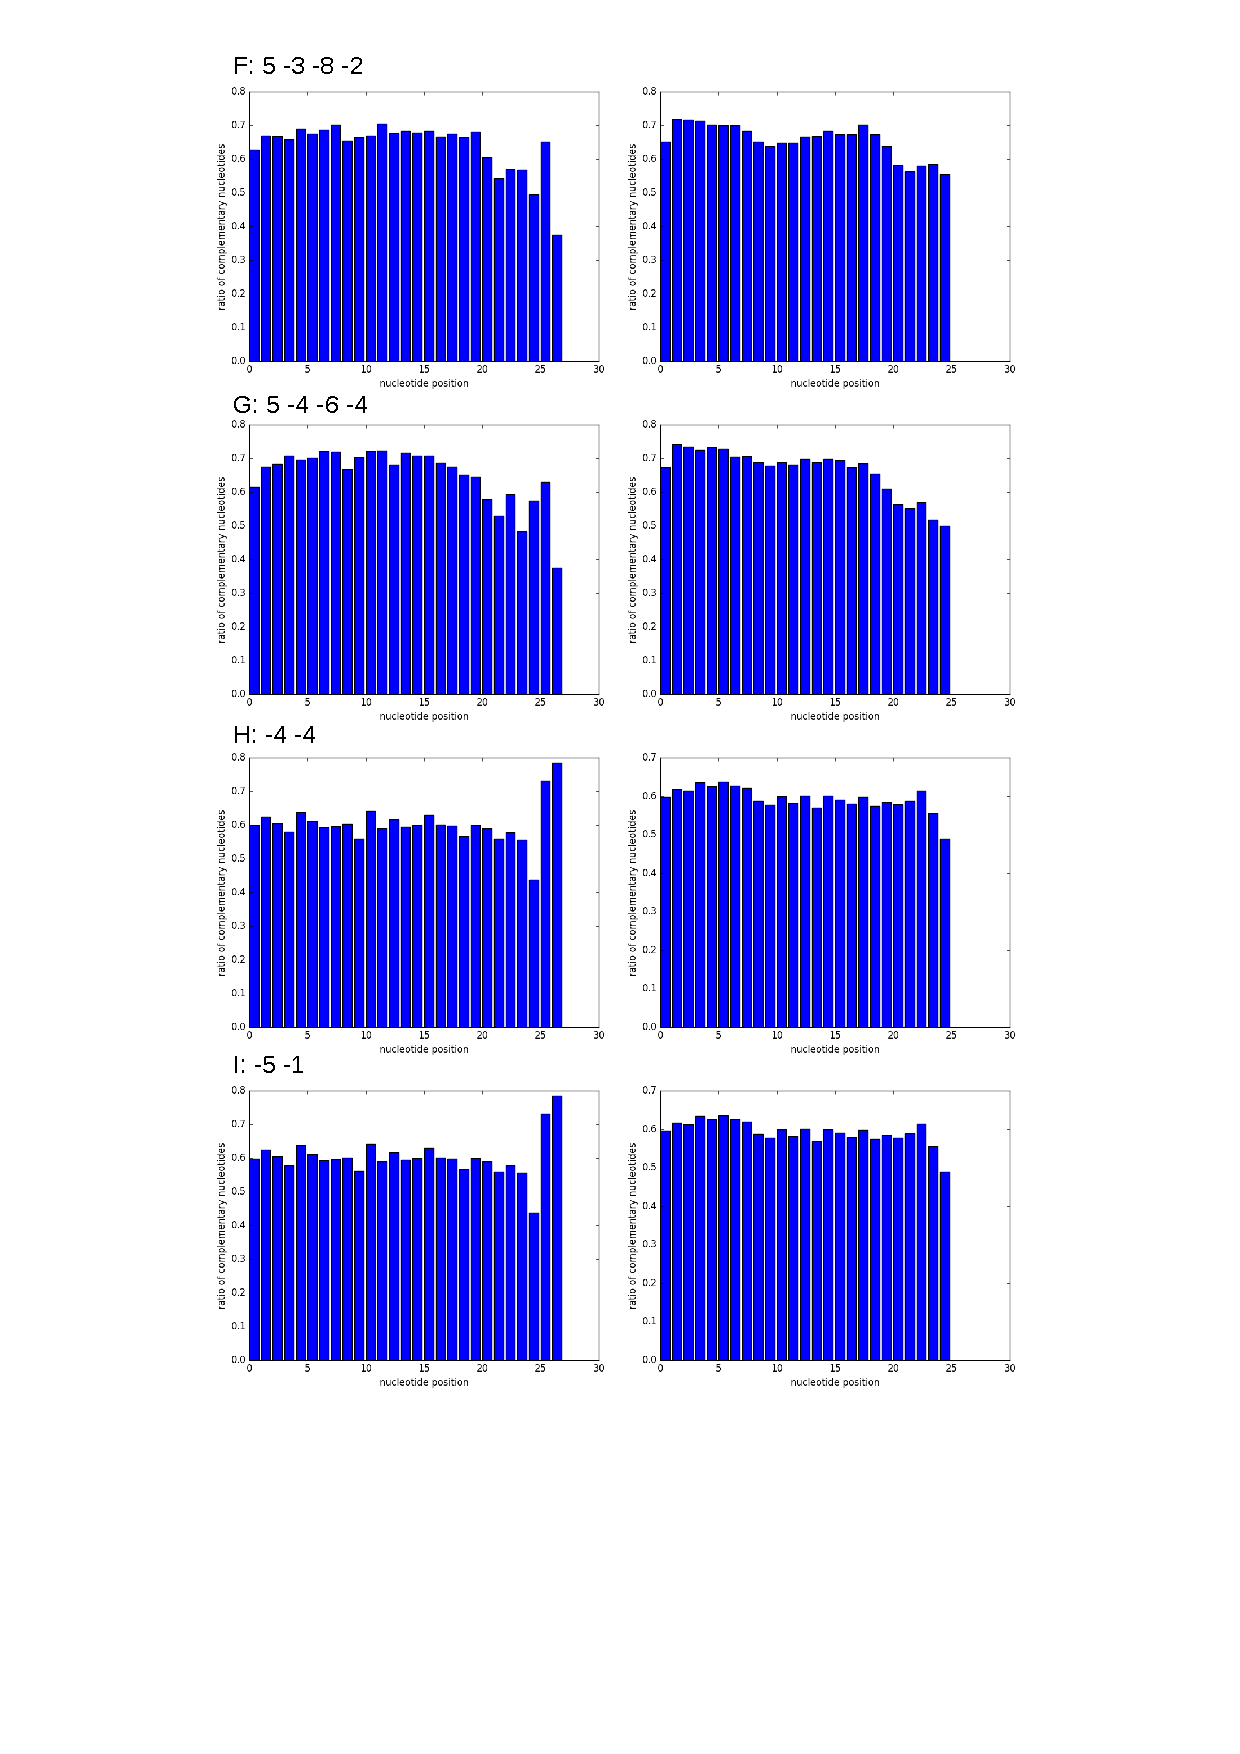
\includegraphics[scale=0.65]{results/combined_results2.pdf}
\vspace{-4cm}
\caption{Ratios of complementarity per parameter set (A-H): targets right, non targets left}
\label{ratios}
\end{figure}

The x-axis of the plots shows the positions one to 22 or more of the miRNA, the y-axis the ratio of complementary bases at this position considering all alignments produced with these parameters. Because most of the miRNAs are only 22 nucleotides long, I will only focus on these positions because higher positions are very imprecise because of the different lengths.

For some sets there is not a significant difference between true targets and non targets, e.g. in plots H and I. Regarding set A, for the true target right an increase in complementarity in the seed region can be observed. On the other hand the ratio towards the end gets really low down to only 30\% of the bases were complementary to the target sequence. In comparison, the maximum of complementarity of the non targets left is shifted towards the central positions, not showing the typical seed region. Notably the plot of the true targets does not show the complementary region towards the 3' end. The same applies for plot B. Considering the other figures of the complementarities there are no significant differences between the two groups. For the non targets all other plots, especially F to I show no big variability overall. The ratios are pretty similar comparing the positions. For the true targets a slight increase in the first positions can be seen but the increase amounts only to a few percentages.
Also for the non targets the complementarity is almost as high as for the true targets, gaining no reliable information for the prediction. This implicates that the consideration of the complementarities of the miRNA positions is not a significant and reliable prediction feature.\\

The analysis of the alignment starting positions was not really successful and significant. Table~\ref{tab:positions} shows the numbers of the own predicted positions that were also given in the miRTarBase. It can be seen that two sets deliver only half the number of the other (5 -2 -8 -3 and 5 -3 -8 -2). These two sets also use very similar parameters. That shows that the alignment positions strongly depend on the selected parameters. In comparison to the given number of about 3700 provided positions in the miRTarBase the numbers of the respective own found ones are in general not very high. This can be due to the different sizes of the UTRs of the genes. In this research they are from the UCSC website whereas the miRTarBase may use another source. Therefore the sizes can be a bit different resulting in different defined positions, although the alignment would start at the same position. To eliminate these small disagreements, I allowed a window of 10 positions where the starting position can be. So if the provided miRTarBase position is given, the own predicted position is classified as consistent if the position lies in a window of +5 or -5 related to the miRTarBase position. 

Another reason for the inconsistent positions may be, that the tools they used in miRTarBase use better and more specific alignment tools where more parameters can be defined. The pairwise2 module only has 4 parameters and only delivers the alignment with the highest score and no ranking. In the database always the best three alignment positions are given.  \\


\begin{table}
\caption{Number of common alignment starting positions}
\vspace{0.3cm}
\begin{tabular}{c||c|c|c|c|c} 
& 3 -2 -4 -4 & 5 -1 -8 -4 & 5 -2 -8 -3 & 5 -3 -8 -2 & 5 -4 -6 -4  \\
\hline\hline
Found number & 815 & 804 & 388 & 411 & 800\\
\hline
\end{tabular}
\vspace{0.5cm}

\begin{tabular}{c||c|c|c|c}
& 1 -2 -2 -1 & 2 -2 -5 -4 & -4 -4 & -5 -1 \\
\hline\hline
Found number & 882 & 793 & 776 & 845  \\
\hline
\end{tabular}
\label{tab:positions}
\end{table}


The table in figure~\ref{table:ratios} shows that the average of the complementarity ratios are pretty similar comparing true targets with non-targets. Highlighted in yellow are the nucleotides of the seed region, in blue the nucleotides of the additional 3' pairing. Building the average ratios of these regions a possible increase could be observed. For the first parameter set, the true targets show a slight increase in the seed region but a decrease in the additional pairing. So the described feature from above can not be significantly observed. For the same set and the negative control, a constant average can be seen. For almost all true target an increase in the seed region and a decrease in the other region can be observed. For the non targets there are different patterns. E.g. for the third parameter set both regions are increased in contrast to the standard average. For the other sets either no big difference can be seen or both are enriched but never decreased. Going back to the plots, there the seed region in the true targets is slightly more visible than for the non targets. But all in all the differences in here are not very big and significant. Both regions can not be observed as clearly as expected.  

\begin{figure}
\vspace{-3cm}
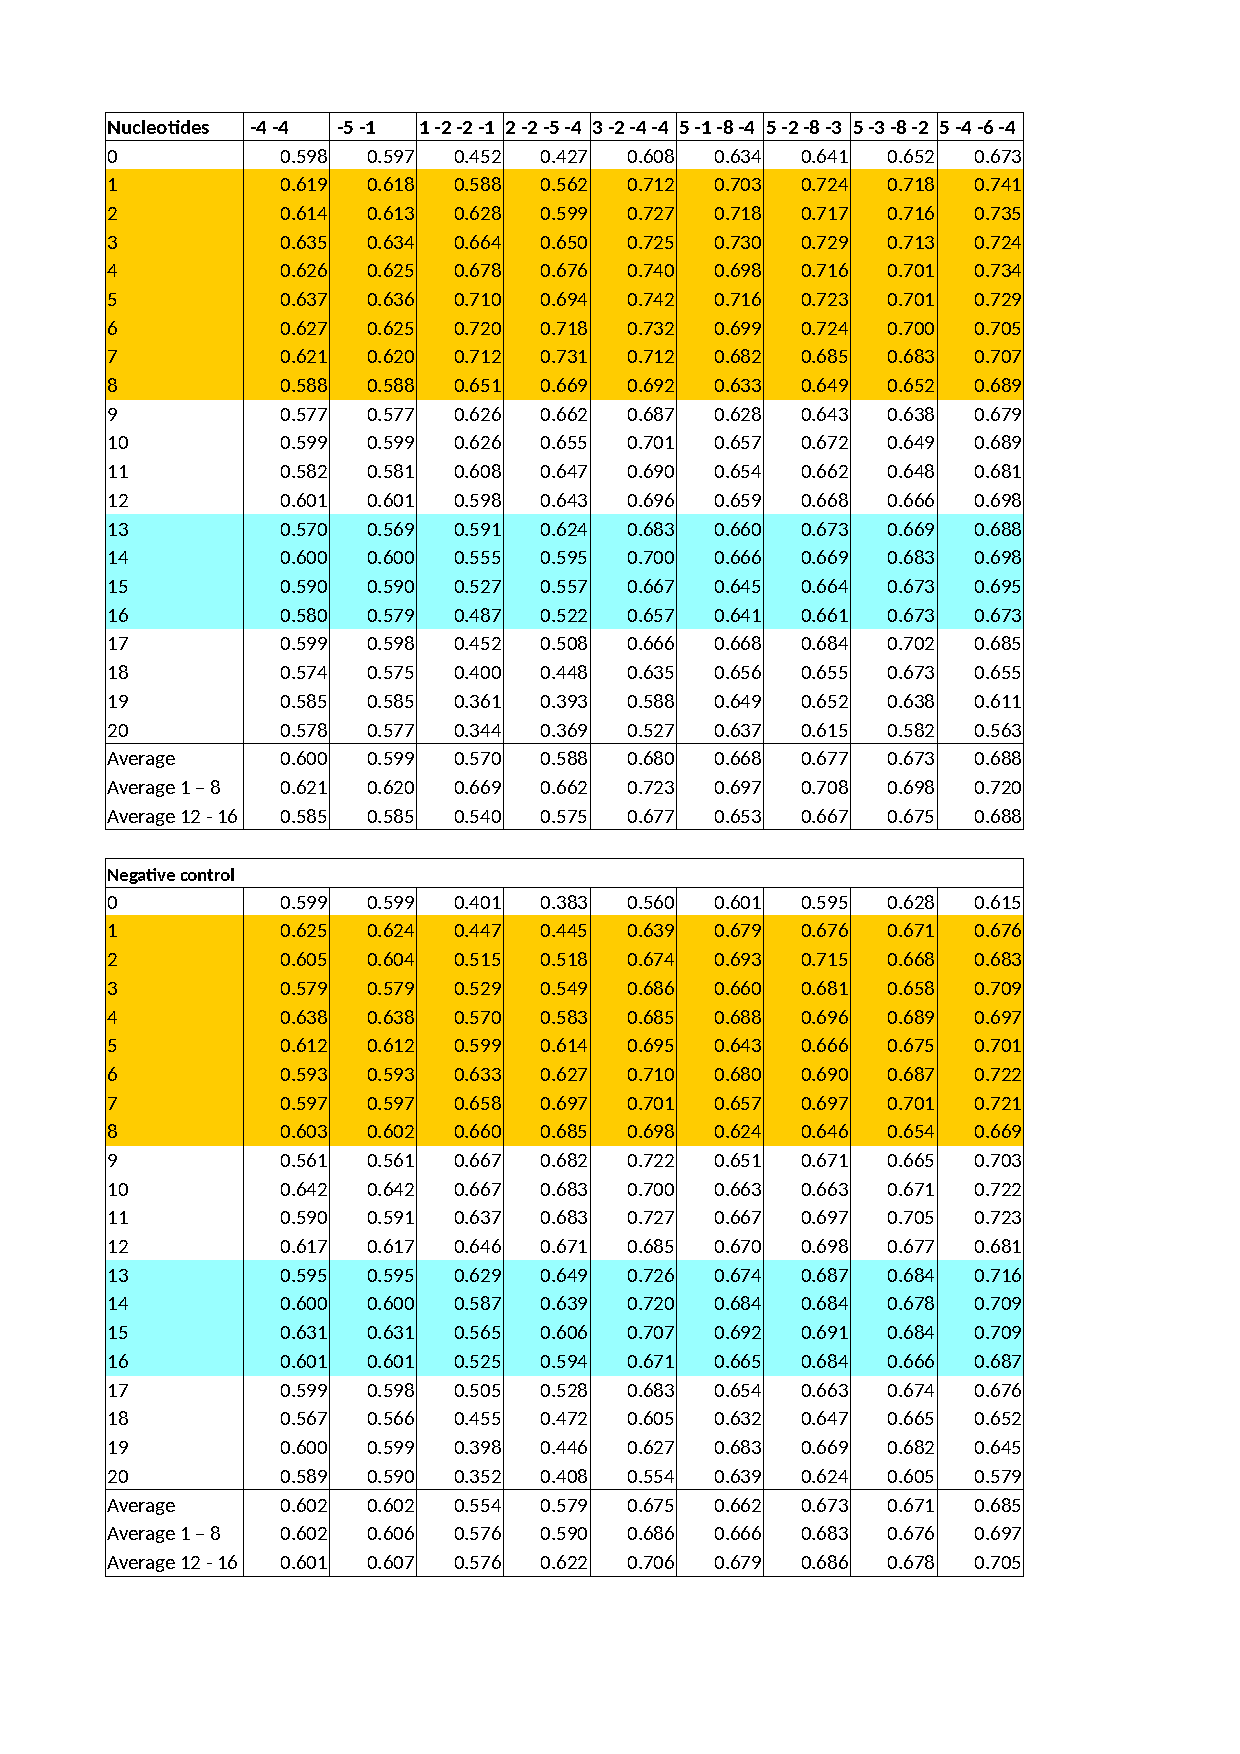
\includegraphics[scale=0.8]{results/ratio_table.pdf}
\vspace{-2.8cm}
\caption{Table of ratios of complementarities}
\label{table:ratios}
\end{figure}



\section{Discussion}
Because of their potential to function in treatment and detection of diseases, miRNAs become more and more important. Therefore miRNA research must be further extended and the complex target prediction has to be improved.


biomarker: http://www.ncbi.nlm.nih.gov/pmc/articles/PMC3199035/

As described above there are many features that can be considered and many different existing tools. They all differ from each other in the number and type of features they use and also in the weighting of the single features \cite{Peterson}. Concluding, each tool and feature has its advantages and strength but also its limitations which makes none of the existing tools perfect and 100\% reliable. 

Relying on just a few features will for sure lead to many errors, either false positives or false negatives. There are many irregularities and some features like the free energy are not always very precise \cite{Peterson}. These problems have to be incorporated to lower the error rate.

Additionally not every tool is frequently updated which is a big problem and does not lead to improvements in target prediction. Some tools do not use the current data or innovations in target interactions. According to Peterson et al. \cite{Peterson} the following tools are outstanding because of maintenance, newest input data and they are the easiest once to use: DIANA-microT-CDS, miRanda-mirSVR and Targetscan. All three are somehow unique but all e.g. use looser thresholds for conservation allowing less conserved regions to balance irregularities and refuse less true targets.

The early miRanda tools is also still widely used. The class of tools that use machine-learning are getting more accurate the more positive and negative target data is verified and features are found. Because of a lack of this data these tools are not significantly better than the three other tools mentioned above \cite{Peterson}.

The future consists of the elimination of the limits the tools and finding more useful features for the prediction.

Fujiwara and Yada \cite{Fuji} followed a new approach by considering other characteristics than binding sites for the prediction, in fact the transcriptional regulation. In their research they searched for common cis-elements in the miRNA as well as in the target gene. Compared to conventional methods theirs method is almost as good as the standard binding site base ones, but combining the two different methods decreases the accuracy much. The advantages of this novel approach are independence of conservation of binding sites and the amount of available training data. 

Coronnello and Benos \cite{Coronnello} investigated another approach trying to improve the prediction power. They developed a tool ComiR that considers additionally the miRNA expression levels and the combination of miRNA bindings. It also combines different scoring schemes from tools mentioned above. The innovation in this tool is the investigation of sets of miRNAs and their co-expression. ?? www.ncbi.nlm.nih.gov/pmc/articles/PMC3692082/




n future die limits die noch da sind zu überwinden um besser zu werden.
New tools: http://www.ncbi.nlm.nih.gov/pubmed/23445489/
combination of tools to overcome limits: http://www.ncbi.nlm.nih.gov/pubmed/23716633/
integrate expression data: http://www.ncbi.nlm.nih.gov/pubmed/23703208/

newst one:http://www.ncbi.nlm.nih.gov/pubmed/27561079
http://www.ncbi.nlm.nih.gov/pubmed/27560313

http://www.ncbi.nlm.nih.gov/pubmed/27494513
  
http://www.ncbi.nlm.nih.gov/pubmed/27477696

http://www.ncbi.nlm.nih.gov/pubmed/27450903

http://www.ncbi.nlm.nih.gov/pubmed/27438777

\newpage
\bibliography{bachelor}


\listoffigures


\listoftables


Figure~\ref{biogenesis}: \cite{Kelly} http://www.nature.com/nrurol/journal/v9/n7/images/nrurol.2012.104-f1.jpg
Figure ~\ref{seed}: http://journal.frontiersin.org/article/10.3389/fgene.2014.00023/full

Figure ~\ref{Fig:canonical}: http://www.targetscan.org/docs/7mer.html

Figure sites: http://www.ncbi.nlm.nih.gov/pubmed/17612493

Table ~\ref{fig:tools}: http://www.ncbi.nlm.nih.gov/pmc/articles/PMC3927079/





\end{document}